\documentclass{article}
\usepackage[margin=3cm]{geometry}
\usepackage{amssymb}

% Figures
\usepackage{graphicx}
\usepackage{color}

% Page formatting
\newsavebox{\notetitle}
\newsavebox{\noteauthor}
\newsavebox{\notenumber}
\newsavebox{\notedate}

\usepackage{url}

%\renewcommand{\title}[1]{\sbox{\notetitle}{\Large{\textbf{#1}}}}
%\renewcommand{\author}[1]{\renewcommand{\and}{\quad}\sbox{\noteauthor}{\large{#1}}}
\renewcommand{\title}[1]{\sbox{\notetitle}{\begin{minipage}{1.0\textwidth} \begin{center} \Large{\textbf{#1}} \end{center}\end{minipage} }}
\renewcommand{\author}[1]{\sbox{\noteauthor}{\begin{minipage}{1.0\textwidth} \begin{center} \large{#1} \end{center}\end{minipage}}}
\renewcommand{\date}[1]{\sbox{\notedate}{\large{#1}}}
\newcommand{\nb}[1]{\sbox{\notenumber}{\Large{\textbf{#1}}}}

\newcommand{\makemadtitle}{
  \hrule
  \vspace{.5em}
  \noindent
  \begin{center}
  \textbf{
  {\centering
\includegraphics[height=3cm,bb=0 0 371 145]{../fig/logoCHISTERA2014.png}}\\
   {\centering\Large COACHES project, CHIST-ERA 2014 program}
  }
  \end{center}
  \vspace{.5em}
 
  \hrule
  \vspace{3em}
  \begin{center}
    %\begin{large}\textbf{ Note~\usebox{\notenumber}.}\end{large}\\[.5em]
    \begin{Large}\textbf{\usebox{\notetitle}}\end{Large}\\[2em]
    \begin{large}\usebox{\noteauthor}\\ [2em]
    \usebox{\notedate}\end{large}
  \end{center}
  \vspace{3em}
}

% Various macros and environments
\newtheorem{prop}{Proposition}
\newtheorem{proposition}[prop]{Proposition}
\newtheorem{defn}{Definition}
\newtheorem{definition}[defn]{Definition}
\newtheorem{cor}{Corollary}
\newtheorem{corollary}[cor]{Corollary}
\newtheorem{exmp}{Example}
\newtheorem{example}[exmp]{Example}
\newtheorem{lem}{Lemma}
\newtheorem{lemma}[lem]{Lemma}
\newtheorem{fact}{Fact}
\newtheorem{thm}{Theorem}
\newtheorem{theorem}[thm]{Theorem}
\newtheorem{prob}{Problem}
\newtheorem{problem}[prob]{Problem}
\newtheorem{rem}{Remark}
\newtheorem{remark}[rem]{Remark}
\newtheorem{conj}{Conjecture}
\newtheorem{conjecture}[conj]{Conjecture}
\newenvironment{pf}{{\bf Proof }}{\hfill$\Box$\par}
\newenvironment{proof}{{\bf Proof }}{\hfill$\Box$\par}
\newcommand{\spaceafterproof}{\vspace{1em}}

% NOTE ITSELF BELOW %%%%%%%%%%%%%%%%%%%%%%%%%%%%%%%%%%%%%%%%%%%%%

\title{D5.2-Sapienza\\ Definition of the use cases for the demonstrations}

\author{Domenico D. Bloisi, Fabio Maria Carlucci, Giorgio Grisetti, \\
Luca Iocchi, and Daniele Nardi\\
\textit{Dept. of Computer, Control and Management Engineering\\
Sapienza University of Rome\\
via Ariosto, 25 00185 Rome, Italy}}


%\nb{of the kickoff meeting, $27^{th},28^{th}$ October }

\date{Version 1.1 - March 26, 2015}

\begin{document}


\includegraphics[height=3cm]{../fig/logoSapienza.png}

\makemadtitle

\begin{abstract}
This document describes the scenario in which the robots will operate and a set of use cases that will be implemented, demonstrated and evaluated.  
\end{abstract}

\vspace*{2.0cm}

\fbox{
\begin{minipage}{1.0\textwidth}
\begin{center}
 $\copyright$, THE COACHES CONSORTIUM \\
The copyright in this document is the property of the COACHES Consortium. This document is supplied by the COACHES consortium on the express terms that it is to be treated as confidential. This document is not external distribution without the project manager's permission. 
\end{center}
\end{minipage}
}
\newpage

\section{Introduction}

COACHES project aims at developing a prototype robotic system for user assistance in a shopping mall.
The COACHES robots will use different modalities, i.e., speech and displayed information,
to interact with the mall visitors, shopkeepers and mall managers.

The scenario where the COACHES robots and systems will be deployed is provided
by the mall ``Rives de l'Orne'', located in the city of Caen, France.

A set of use cases will be implemented to show the feasibility of the approach and to assess the effectiveness of the proposed solutions with actual users.
In particular, this document contains:
\begin{enumerate}
\item A brief description of the test facilities;
\item The descriptions of four use cases that focus on two main components of the entire system,
namely short-term human-robot interaction and safe navigation.
\end{enumerate}

\section{Test facilities: Collaboration with the Mall Rives de l'Orne}

\begin{figure}[!t]
\begin{center}
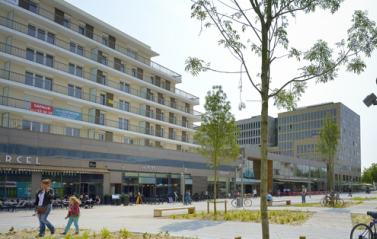
\includegraphics[width=0.55\linewidth]{outsiderivesdelorne}
\caption{The mall Rives de l'Orne.}
\label{fig:outsidemall}
\end{center}
\end{figure}

The test facilities concerns the mall ``Rives de l'Orne'' (see Fig. \ref{fig:outsidemall}). Rives de l'Orne\footnote{\url{http://www.rivesdelorne.com}} is a 
new and modern mall
situated in the city of Caen (France). It is composed of two face-to-face buildings separated by a large
main square (see Fig. \ref{fig:map}). At the first floor of the two buildings, there are many shops and restaurants. In the main square, there is a cinema. This space is surrounded by tramway stations and a train station.

\begin{figure}[!t]
\begin{center}
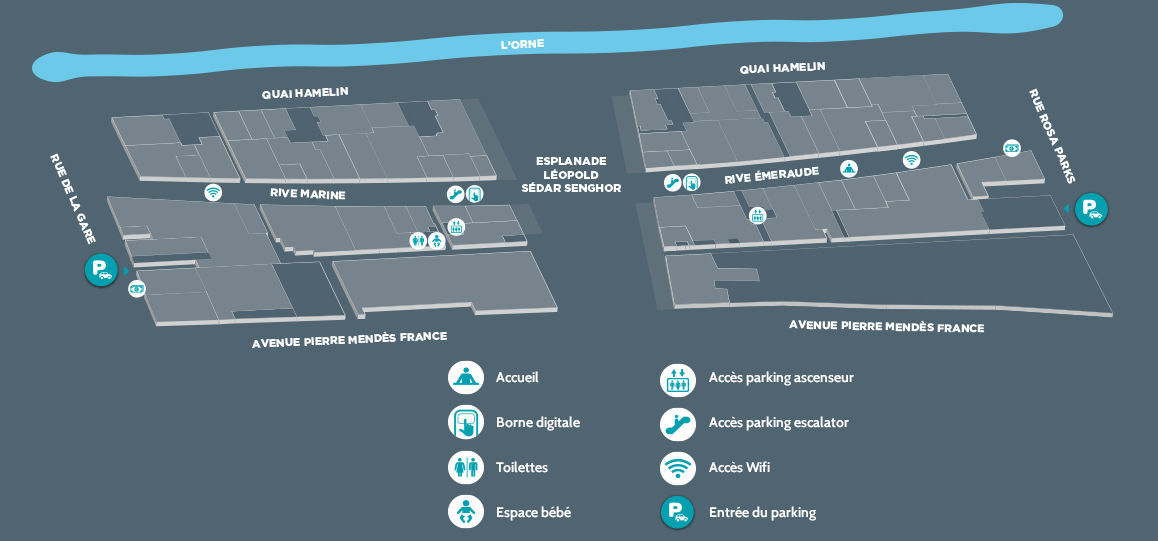
\includegraphics[width=1.0\linewidth]{mallplan}
\caption{The map of the mall.}
\label{fig:map}
\end{center}
\end{figure}

The mall is visited by more than 100,000 customers every year. In addition to customers,
several elderly people
live in the apartments located at the other floors of the buildings. These people have their habit and there are frequent customers of the mall (see Fig. \ref{fig:insidemall}).

\begin{figure}[!t]
\begin{center}
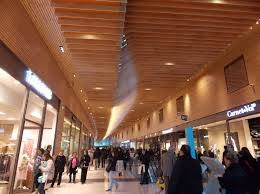
\includegraphics[width=0.5\linewidth]{InsideRivedelOrne}
\caption{Inside the mall Rives de l'Orne.}
\label{fig:insidemall}
\end{center}
\end{figure}

Two meetings have been organized ($23^{th}$ October 2014 and $12^{th}$ December 2014) to define the equipment to be installed, in terms of cameras and sensors.
Regarding the sensors, Radio-Frequency IDentification (RFID) tags and receivers will be used.
Cameras and sensors are in charge of sending information to the COACHES robots
about
\begin{itemize}
\item the shops;
\item the planning of the robot deployment in the mall;
\item the scheduled dissemination actions.
\end{itemize}

A visit of all COACHES project partners have been organized during the kickoff meeting,
held on $27^{th}$ and $28^{th}$ October 2014 in Caen. 


\section{Use cases for short-term interaction and navigation}

COACHES project envisages the implementation of a set of use cases
to show the feasibility of the approach and to assess the effectiveness
of the proposed solutions with actual users.
To this end, different use cases will be implemented, focusing on two main
components of the entire system:
\begin{enumerate}
\item Short-term human-robot interaction;
\item Safe navigation.
\end{enumerate}

Four use cases are described in the following. The use case are designed
to allow a short-term interaction between the COACHES robot and the human users.
In order to accomplish the required tasks, the robot must navigate
safely the environment. Navigation inside a populated environment, i.e., a mall
during opening hours, must be done in order to avoid damage to people
and goods.

For each use case, the following data are provided:
\begin{itemize}
\item A brief textual description;
\item One (or more) sequence diagrams;
\item An optimistic sequence of actions.
\end{itemize}

Furthermore, a detailed overview of the preconditions and post-conditions for each
used action is given at the end of this section.


\subsection{Customers ask for help carrying bags}

The objective of this use case is to highlight the social awareness
of the robot in the completion of a given task. There are many ways
to carry a bag for a customer, but only a few might be socially acceptable
at a given moment. To perform good, the robot asks the customer about her/his priorities.

\subsubsection{Use case description}

The robot is called by a shop manager (or by a customer) to help
in carrying bags. Bag loading operations take place in dedicated areas,
located at the exit of the shops.
The robot has to
\begin{enumerate}
\item Reach the exit of the shop;
\item Approach the dedicated bag loading area.
\end{enumerate}

\noindent When in position, the robot waits for the customer to establish
a contact.
Once the customer has established a contact, the robot asks the user
to load the bag in the bin carried by the robot.
Once the bag is loaded, the robot asks the customer if she/he is in a hurry.
If the customer is in a hurry, the robot
\begin{enumerate}
\item sets its speed to an high value;
\item proceeds to the mall parking lot.
\end{enumerate}

\noindent In the other case, the robot
\begin{enumerate}
\item sets its speed to a low value;
\item proceeds to the mall parking lot, proposing intermediate stops to shops
with interesting discounts.
\end{enumerate}

In any case the robot modulates its speed taking into account the number of detected people,
to minimize the risk of collision.

\subsubsection{Sequence diagram}

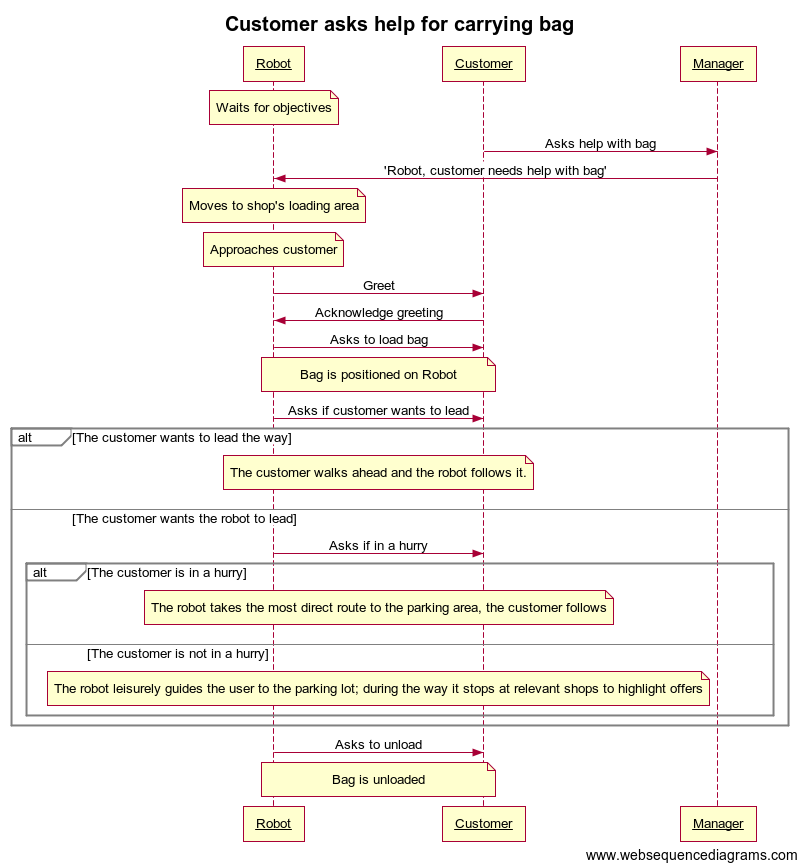
\includegraphics[width=0.85\textwidth]{bagUseCase}


\subsubsection{Optimistic robot action sequence}
\begin{enumerate}
\item Go to shop's loading area
\item Approach customer
\item Start conversation
\item Ask to load bag
\item Ask if customer wants to lead
\item Follow customer
\item Ask To Unload
\item End conversation
\end{enumerate}


\subsection{Proposing an ice cream to a child}

This use case serves to demonstrate the common sense reasoning capability
of the robot. Since it is not socially acceptable for the robot to guide
a child to a location without her/his parents permission, the robot
asks for the parent's permission before completing the task.

\subsubsection{Use case description}

The manager of an ice cream shop asks the robot to inform children about
a special discount. The robot looks around for children. When it detects
a child, the robot approaches her/him and it informs her/him
about the special discount. The child
is passionate about having an ice cream, but before guiding her/him
to the ice cream shop, the robot
\begin{enumerate}
\item asks for the parent's authorization.
\item waits for the positive parent's reply.
\end{enumerate}

\noindent Once the parent agrees to allow the child to follow the robot, it proceeds
to the ice cream shop.

\subsubsection{Sequence diagrams}

\begin{figure}[!h]
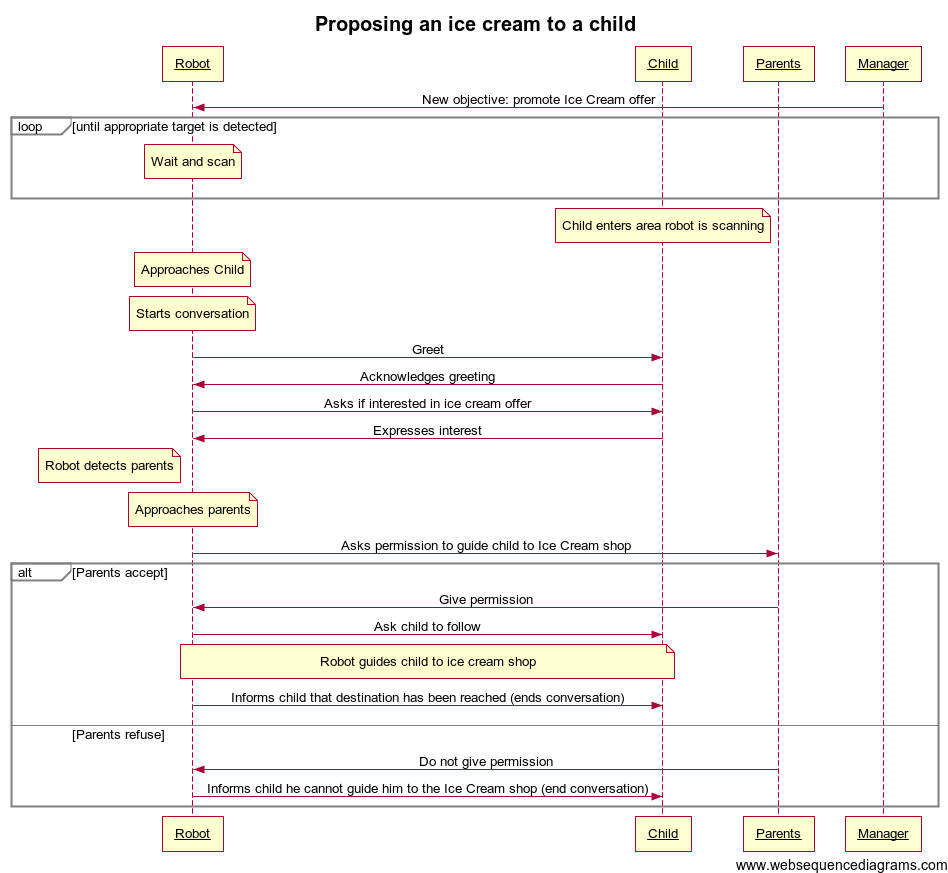
\includegraphics[width=0.85\textwidth]{iceCreamA}
\protect\caption{Option A: Parents are near the child.}
\end{figure}


\begin{figure}[!h]
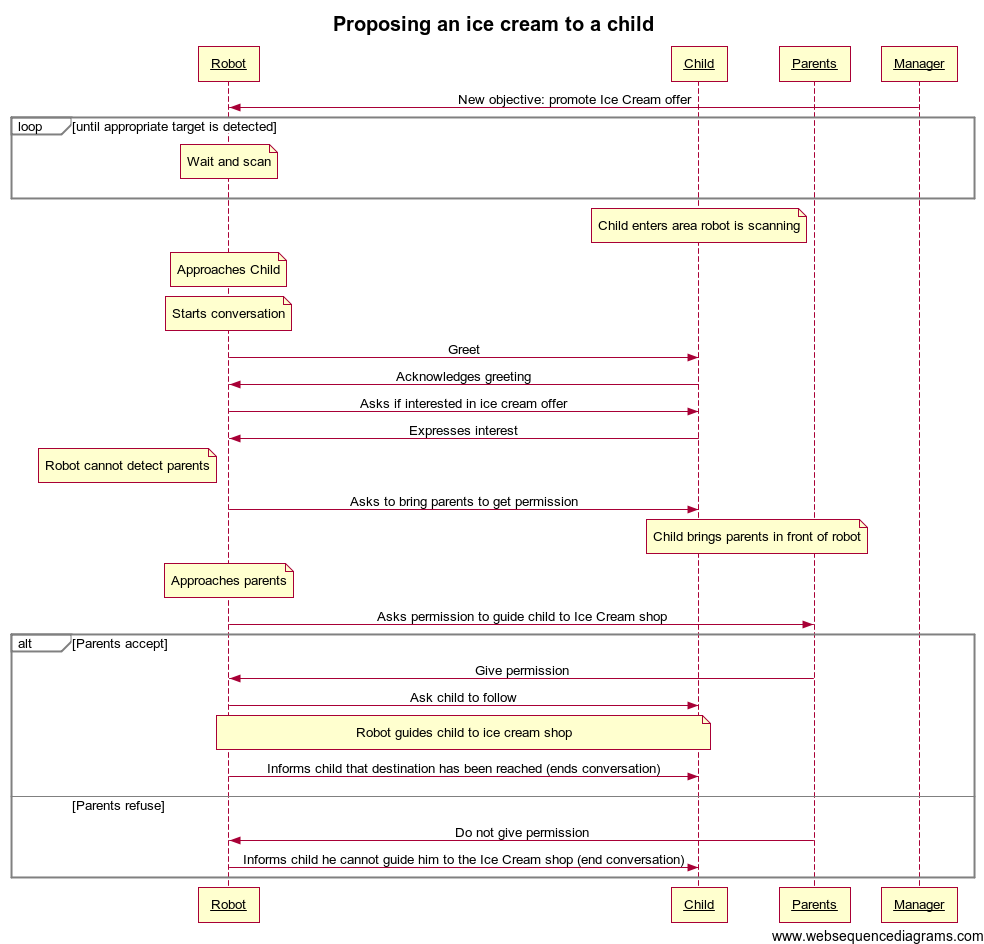
\includegraphics[width=0.85\textwidth]{iceCreamB}
\protect\caption{Option B - Parents are not near the child.}
\end{figure}



\subsubsection{Optimistic robot action sequence}
\begin{enumerate}
\item Approach child
\item Start conversation
\item Offer ice cream discount
\item Ask parents for permission
\item Ask child to follow
\item Go to IceCreamShop
\item Inform customer destination has been reached
\item End conversation
\end{enumerate}

\newpage

\subsection{Customer refuses the first robot proposal and accepts a different one}

This use case highlights how the robot is capable of
recovering from a failure by exploiting automatic reasoning.
Since the customer refuses the first offer proposed by the robot, it, instead of randomly proposing 
a new offer to her/him, tries to understand the user's preferences.

Moreover, in this use case, the proactive nature of the robot's behavior (when allowed by security
concerns) is also underlined: When no people are
moving around, the robot can decide to approach itself a potential
customer.

\subsubsection{Use case description}

The sales manager of a cinema inside the mall needs to promote a special discount
for a movie. The discount is loaded by the manager into the 
knowledge base (KB) of the robot, that contains the list of all the active commercial offers.
The robot is also aware, in his persistent KB, of the
existence of other secondary discounts.

Since there are no people moving around the robot, it starts
waiting for customers by monitoring the scene. As soon as the robot
sees a potential user (moving at the right distance and at the right speed),
the robot intercepts the customer and it asks her/him if she/he is interested
in the special discount for the movie.

The user answers that she/he is not interested.
Then, the robot asks the user to slide her/his personal customer card in order to
obtain a different available discount, in accordance to the user's previous purchases.

After the card data has been read, the robot finds out that the customer is a woman and that she
has made many purchases in the personal care department. 
Thus, the robot, by analysing the list of all the active commercial offers,
infers that the special discount about a facial cream could be of interest
to her.

Once informed of the discount, the customer reveals
that she is interested in it and she asks the robot for directions to reach the specific
shop. The robot safely guides the customer to the shop.

\newpage

\subsubsection{Sequence diagram}

\begin{figure}[!h]

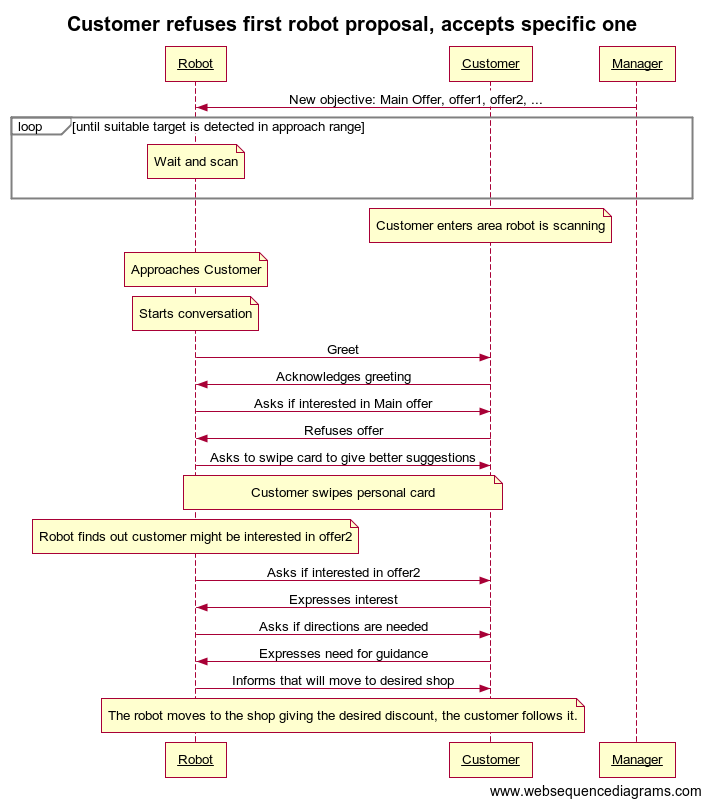
\includegraphics[width=0.75\textwidth]{offerReasoning}

\end{figure}



\subsubsection{Optimistic robot action sequence}
\begin{enumerate}
\item Approach customer
\item Start conversation
\item Propose main offer (in this use case we assume this fails)
\item Ask for the customer to identify himself by swiping the card
\item Find appropriate offer for user
\item Propose new offer to user
\item Ask customer to follow
\item Go to appropriate shop
\item Inform customer destination has been reached
\item End conversation
\end{enumerate}


\subsection{Customer asks for directions in a crowded environment}

The goal of this use case is to remark that the robot must always be
aware of safety. The robot is not allowed to behave hazardously
in presence of humans.

\subsubsection{Use case description}

The robot has the objective to inform customers of available discounts.
The shopping mall is very crowded and, for safety
reasons, the robot decides that it should not move around, but
that is more convenient to wait
for users to approach it.

As soon as it detects a user, standing still at
the appropriate social distance and looking at her/him, the robot initiates
a conversation and it announces the available offers.

The user is interested in a listed offer
and she/he asks for directions to reach the shop offering a discount.
Since the robot cannot safely move due to the crowded environment, it
\begin{enumerate}
\item shows the user the desired path on its tablet;
\item informs the user that 20 meters away along the corridor she/he will find another robot,
that can provide more specific information, if needed.
\end{enumerate}

\noindent The human thanks the robot and proceeding to the next one in order to
receive further directions.

\subsubsection{Sequence diagrams}

\begin{figure}[!h]
\fbox{\begin{minipage}[t]{0.48\columnwidth}%
\begin{center}
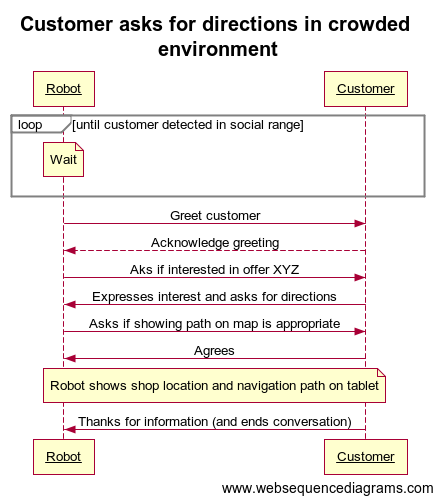
\includegraphics[width=1\textwidth]{crowdedCaseA}
\par\end{center}

\begin{center}
\textit{Robot shows path on map}
\par\end{center}%
\end{minipage}}\hfill{}%
\fbox{\begin{minipage}[t]{0.48\columnwidth}%
\begin{center}
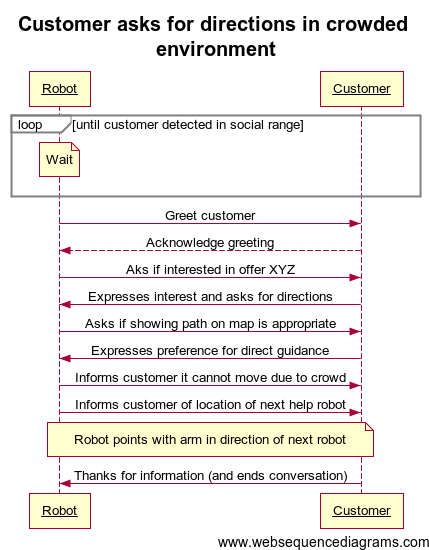
\includegraphics[width=1\columnwidth]{crowdedCaseB}
\par\end{center}

\begin{center}
\textit{Robot shows where next helper is}
\par\end{center}%
\end{minipage}}

%\protect\caption{Customer asks for directions in crowded environment}


\end{figure}



\subsubsection{Optimistic robot action sequence}

\textit{A human approaches the robot}
\begin{enumerate}
\item Start conversation
\item Ask if interested in offer XYZ
\item Ask if showing path on map is appropriate
\item Show path to shop on tablet
\item End conversation
\end{enumerate}

\section{Robot actions}

In this section, the actions that the robot has to perform in order to
accomplish its tasks are described.
For each action, the preconditions and the post conditions that must hold are
listed. 


\subparagraph{Approach Human(Human)}

:

\textit{Prec}: The human has been detected by sensors and is reachable.

\textit{Post}: The robot positions itself at a social distance from
the user, possibly in plain view and facing the human.

\textit{Description}: This action usually precedes starting a conversation


\subparagraph{AskHumanIfInHurry(Human)}

:

\textit{Prec}: The robot is carrying something belonging to the human,
the human asked to robot to lead

\textit{Post}: The fact that the human is in a hurry or not, is added
to the knowledge base.

\textit{Description}: This question is asked to understand if the
robot should move directly to the parking area or can show a few offers
during the way


\subparagraph{AskHumanToDeload(Human)}

:

\textit{Prec}: The robot is carrying something belonging to the human

\textit{Post}: The human's object is removed from the robot

\textit{Description}: If the human refuses to remove the object, a
manager should be notified.


\subparagraph{AskHumanToLoad(Human)}

:

\textit{Prec}: The robot is in conversation with the human

\textit{Post}: The human's bag is on top of the robot

\textit{Description}:


\subparagraph{AskHumanWhoLeads(Human)}

:

\textit{Prec}: The robot is carrying something belonging to the human

\textit{Post}: The fact that the human wants to lead, or the contrary,
is added to the knowledge base.

\textit{Description}: This question is asked to understand if the
robot must lead or follow the human

 


\subparagraph{End Conversation(Human)}

:

\textit{Prec}: Human and robot are engaged in conversation.

\textit{Post}: Human and robot are no longer engaged in conversation.

\textit{Description}: The robot follows a social protocol to end the
conversation (es: ``See you next time!'')


\subparagraph{Engage Conversation(Human)}

:

\textit{Prec}: Robot is in social range with human. Human can see
robot, robot is facing human.

\textit{Post}: Human and robot are engaged in conversation.

\textit{Description}: The robot follows a social protocol to start
the conversation (``Hello human'') and make sure the human is interested


\subparagraph{Goto(Destination)}

:

\textit{Prec}: There is a path to the destination.

\textit{Post}: The robot is now at(Destination)

\textit{Description}: The robot navigate in a socially aware way to
the desired location.





\end{document}
